\chapter[Extended Study: Task and Morphology Dependence]{Extended Study: Task and\\Morphology Dependence}
\label{cha:extended}

\section{Motivation and Research Question}
\label{sec:extended-motivation}

The original study establishes that \nchl{} can evolve useful behaviour, but its small task set cannot show whether performance follows a general task property. The extended study addresses the limitations by comparing \nchlcontroller{} and Static-ES on twelve tasks and three controlled bodies.

This experiment answers RQ4: \emph{which task characteristics are associated with good \nchl{} performance, and are those patterns independent of morphology?} The chapter first reports the predefined group comparison and then uses individual tasks to interpret the physical and temporal demands behind it.

\section{Experimental Design}
\label{sec:extended-design}

\subsection{Task Selection and Predefined Groups}

The twelve environments were assigned to four groups before their results were inspected (\Cref{tab:extended-task-groups}). The groups describe a dominant control demand.

\begin{table}[htbp]
  \centering
  \small
  \caption{Predefined task groups in the extended experiment.}
  \label{tab:extended-task-groups}
  \begin{tabularx}{\textwidth}{@{}>{\raggedright\arraybackslash}p{0.22\textwidth}>{\raggedright\arraybackslash}p{0.35\textwidth}>{\raggedright\arraybackslash}X@{}}
    \toprule
    Group & Tasks & Dominant characteristic \\
    \midrule
    Continuous-support locomotion & Walker; BridgeWalker; BidirectionalWalker & Repeated locomotion on rigid or deformable support, including changing goals \\
    Terrain negotiation & DownStepper; ObstacleTraverser; CaveCrawler & Contact adaptation, terrain sensing, step transitions, and clearance control \\
    Object interaction & Pusher; Carrier; Thrower & Control while mechanically coupled to an external object \\
    Whole-body dynamic control & Flipper; Jumper; Balancer & Rotation, impulse generation, or postural regulation without sustained transport \\
    \bottomrule
  \end{tabularx}
\end{table}

\subsection{Control Demands of the Individual Tasks}

The group labels conceal differences that may matter to an activity-dependent controller. Based on the objectives and mechanics of the EvoGym environments, \Cref{tab:extended-task-demands} gives the author's classification of the principal temporal and physical demand of every task~\cite{bhatia2021evolution}. In particular, a repetitive task can retain one objective, as in Walker, or require repeated goal changes, as in BidirectionalWalker. Likewise, object interaction can require sustained contact or one precisely timed release.

\begin{table}[htbp]
  \centering
  \scriptsize
  \caption{Task characteristics used to interpret the controller comparison.}
  \label{tab:extended-task-demands}
  \begin{tabularx}{\textwidth}{@{}l>{\raggedright\arraybackslash}p{0.27\textwidth}>{\raggedright\arraybackslash}X@{}}
    \toprule
    Task & Temporal structure & Principal physical or control demand \\
    \midrule
    Walker & Repeated, fixed direction & Locomotion on rigid continuous support \\
    BridgeWalker & Repeated, fixed direction & Locomotion coupled to deformable support \\
    BidirectionalWalker & Sequential goals & Direction changes and context-dependent action \\
    DownStepper & Repeated with transitions & Descending contacts while remaining upright \\
    ObstacleTraverser & State-dependent & Terrain sensing, clearance, and balance \\
    CaveCrawler & Repeated under constraint & Simultaneous floor and ceiling clearance \\
    Pusher & Sustained progression & Persistent contact with a movable object \\
    Carrier & Sustained progression & Transport while retaining the load \\
    Thrower & Phase structured & Load, accelerate, and release \\
    Flipper & Repeated, one direction & Continued whole-body rotation \\
    Jumper & Ballistic & Compression, launch, and height retention \\
    Balancer & Stabilizing & Approach and maintain a target state \\
    \bottomrule
  \end{tabularx}
\end{table}

\subsection{Controlled Morphologies}

Every task is evaluated with a generalist biped, compact crawler, and hollow frame. Each body contains 24 occupied voxels: 12 rigid, two soft, five horizontal actuators, and five vertical actuators. The action dimension is therefore ten in every condition. Geometry and mass distribution change, while occupied volume, material counts, and actuator budget remain fixed.

\begin{figure}[htbp]
  \centering
  \begin{subfigure}[t]{0.31\textwidth}
    \centering
    \setlength{\tabcolsep}{0pt}
    \begin{tabular}{cccccc}
      \emptyvoxel&\rigidvoxel&\rigidvoxel&\rigidvoxel&\rigidvoxel&\emptyvoxel\\
      \hactvoxel&\vactvoxel&\rigidvoxel&\rigidvoxel&\hactvoxel&\vactvoxel\\
      \rigidvoxel&\hactvoxel&\softvoxel&\softvoxel&\vactvoxel&\rigidvoxel\\
      \vactvoxel&\hactvoxel&\emptyvoxel&\emptyvoxel&\vactvoxel&\hactvoxel\\
      \rigidvoxel&\rigidvoxel&\emptyvoxel&\emptyvoxel&\rigidvoxel&\rigidvoxel
    \end{tabular}
    \caption{Generalist biped.}
  \end{subfigure}
  \hfill
  \begin{subfigure}[t]{0.31\textwidth}
    \centering
    \setlength{\tabcolsep}{0pt}
    \begin{tabular}{cccccc}
      \rigidvoxel&\rigidvoxel&\rigidvoxel&\rigidvoxel&\rigidvoxel&\rigidvoxel\\
      \hactvoxel&\vactvoxel&\softvoxel&\softvoxel&\hactvoxel&\vactvoxel\\
      \rigidvoxel&\hactvoxel&\rigidvoxel&\rigidvoxel&\vactvoxel&\rigidvoxel\\
      \vactvoxel&\hactvoxel&\rigidvoxel&\rigidvoxel&\vactvoxel&\hactvoxel
    \end{tabular}
    \caption{Compact crawler.}
  \end{subfigure}
  \hfill
  \begin{subfigure}[t]{0.31\textwidth}
    \centering
    \setlength{\tabcolsep}{0pt}
    \begin{tabular}{cccccc}
      \emptyvoxel&\rigidvoxel&\rigidvoxel&\rigidvoxel&\rigidvoxel&\emptyvoxel\\
      \hactvoxel&\vactvoxel&\rigidvoxel&\rigidvoxel&\hactvoxel&\vactvoxel\\
      \rigidvoxel&\hactvoxel&\emptyvoxel&\emptyvoxel&\vactvoxel&\rigidvoxel\\
      \vactvoxel&\hactvoxel&\emptyvoxel&\emptyvoxel&\vactvoxel&\hactvoxel\\
      \rigidvoxel&\rigidvoxel&\softvoxel&\softvoxel&\rigidvoxel&\rigidvoxel
    \end{tabular}
    \caption{Hollow frame.}
  \end{subfigure}

  \medskip
  \voxellegend
  \caption{Controlled morphologies.}
  \label{fig:extended-bodies}
\end{figure}

The biped separates support into leg-like columns, the crawler forms a low and nearly rectangular contact structure, and the frame redistributes the same material around a central opening. 

\subsection{Experimental Scale and Completeness}

The design contains $12\times3\times2\times10=720$ independent optimization runs. Every run completed 500 generations with a population of 40 and mutation scale $0.35$. Static candidates use one episode, while \nchl{} candidates again average three runtime-weight initializations.

\section{Analysis Strategy}
\label{sec:extended-analysis}

The task-level curves first average the three morphology scores within each seed and then summarize the ten independent seeds. Their outcome is best-so-far fitness during evolution. Final comparisons use the selected best-so-far score at generation 500. Footage of the evolved controllers supplies a separate behavioural check: a higher task reward is not treated as evidence of controller capability when the robot is not able to perform the intended task recognizably. Numerical results from such conditions remain reported, but receive little weight.

Raw return is meaningful within a task but cannot be pooled across tasks. For task $t$, morphology $m$, and seed $s$, the controller difference is therefore standardized by the sample standard deviation of the 20 final scores in that task--morphology stratum:
\begin{equation}
  z_{tms}=
  \frac{F^{\nchl}_{tms}-F^{\mathrm{static}}_{tms}}{s_{tm}}.
  \label{eq:extended-standardized-effect}
\end{equation}
Positive values favour \nchlcontroller{} and negative values favour Static-ES. Group effects average the nine standardized values contributed by three tasks and three morphologies within each seed. Means are accompanied by non-parametric bootstrap intervals over the ten seed-level values. Raw within-task differences are retained where standardization could obscure practical magnitude.

\section{Results Across Tasks and Morphologies}
\label{sec:extended-results}

\subsection{Training Dynamics and Task-Group Results}

Both controller representations improve numerically on every task, but they do not reach the same training ceiling (\Cref{fig:extended-training-curves}). Walker, BridgeWalker, Pusher, Jumper, and CaveCrawler show rapid early gains followed by a plateau. Static-ES continues to separate on BidirectionalWalker, DownStepper, ObstacleTraverser, Carrier, Thrower, and Balancer. 

\begin{figure}[htbp]
  \centering
  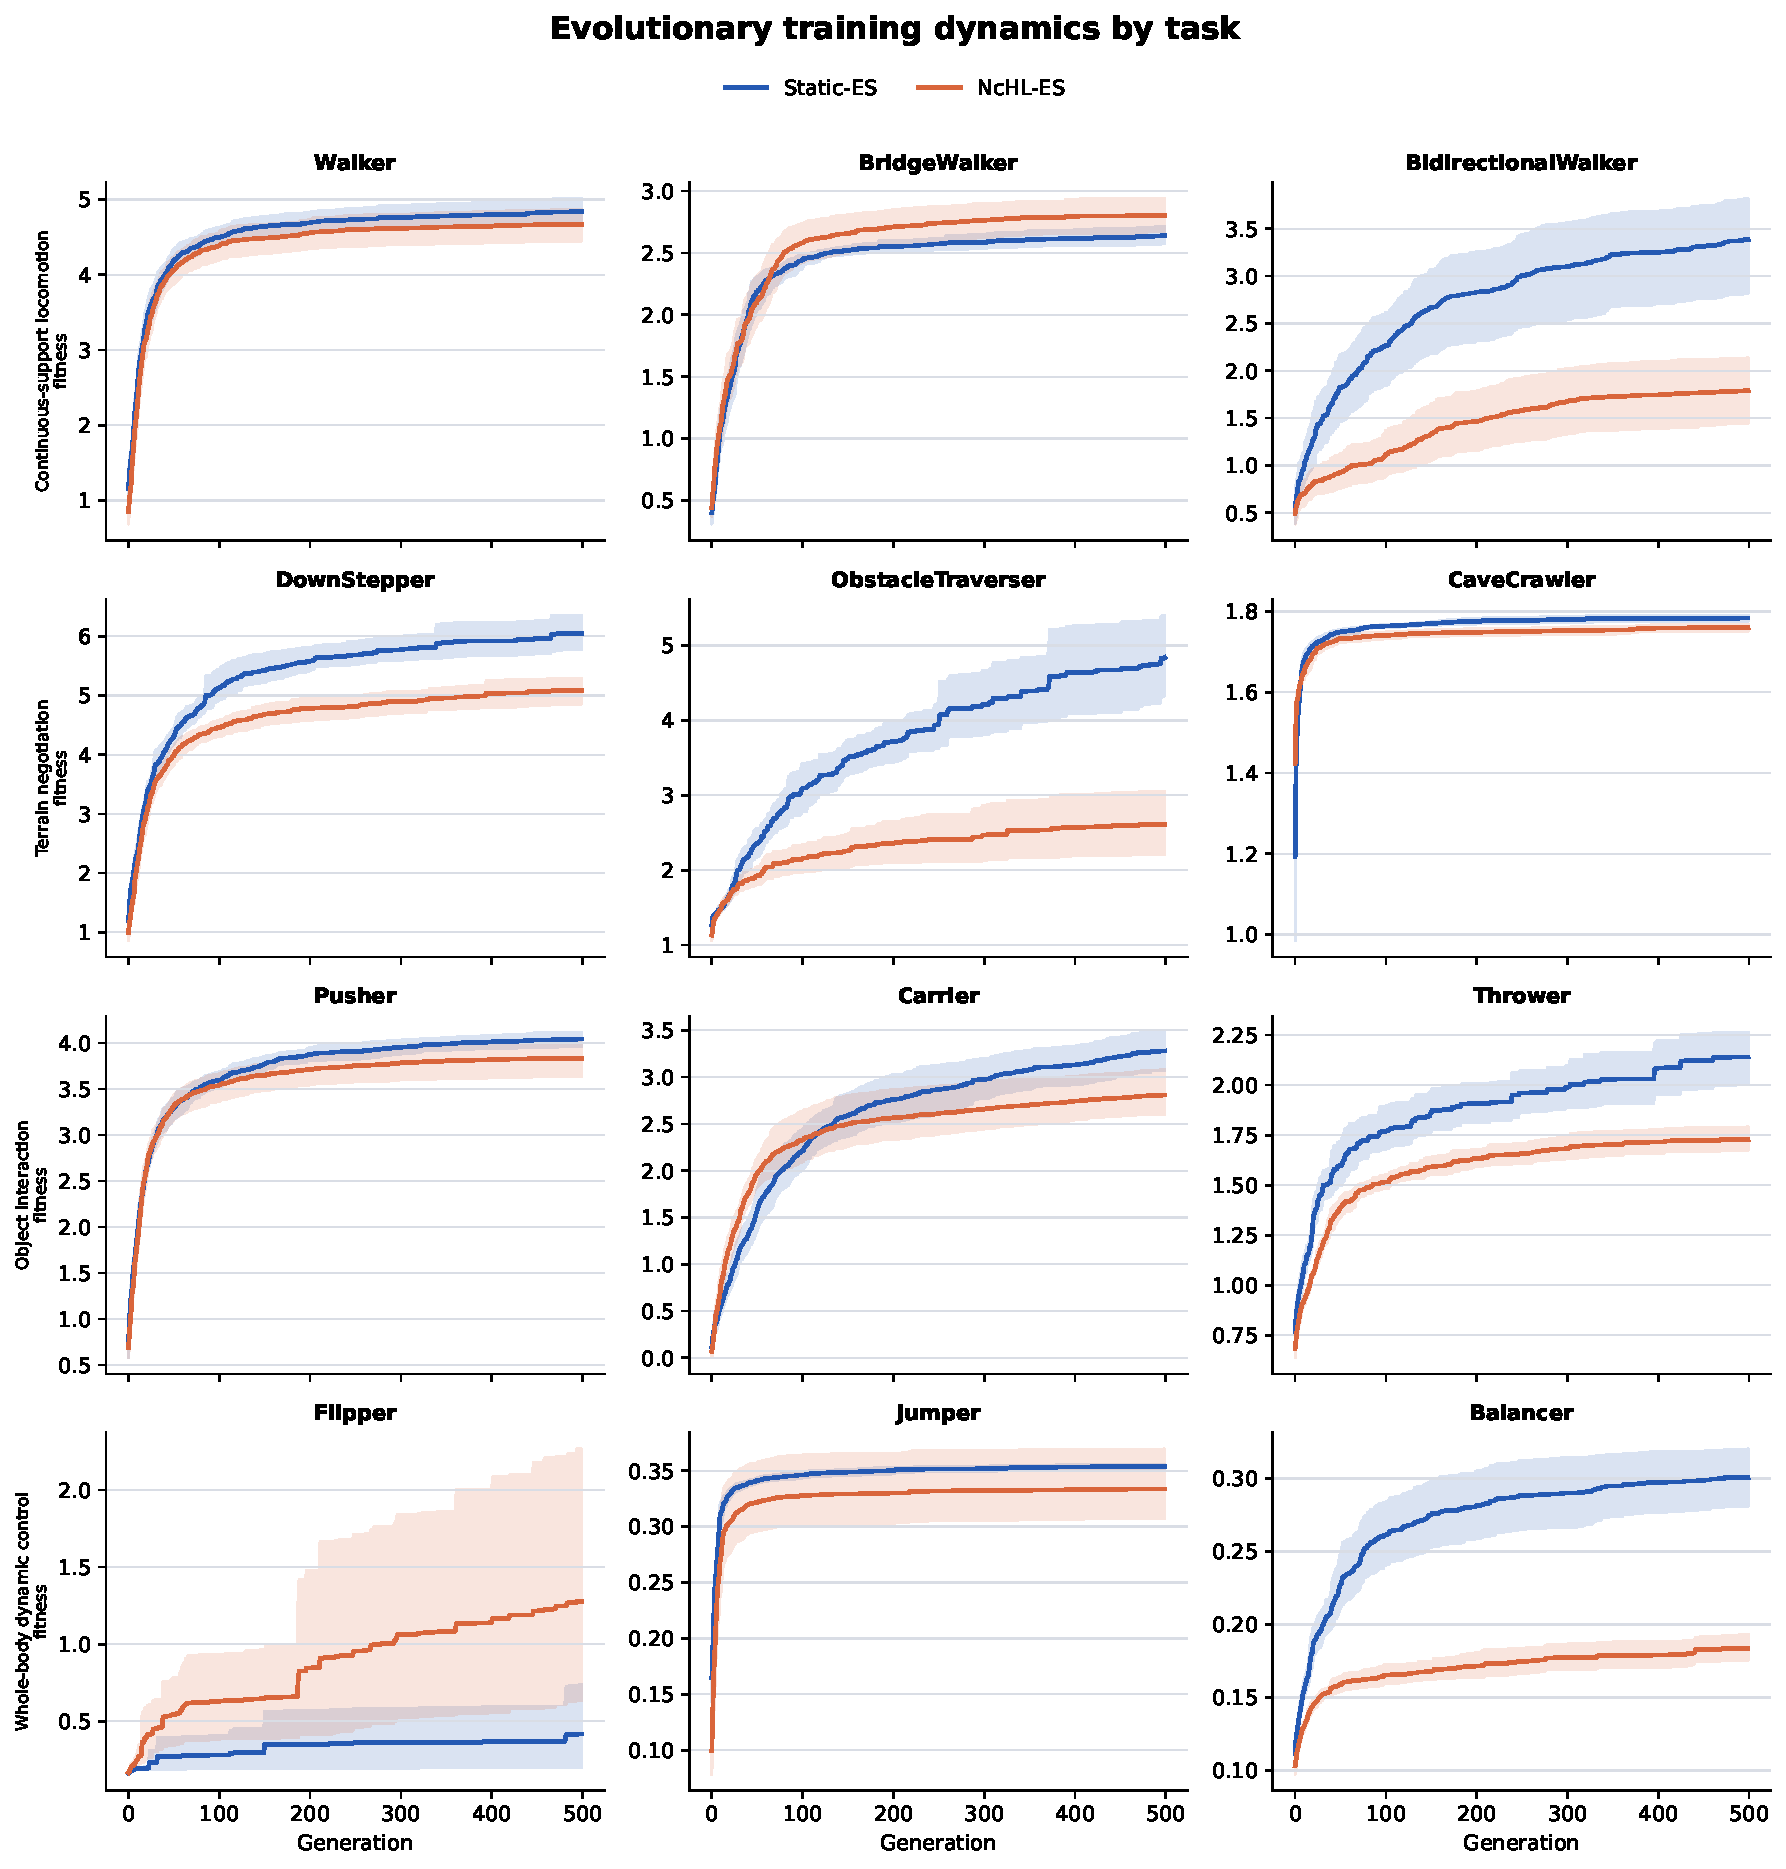
\includegraphics[width=0.98\textwidth]{figures/training_curves_by_task.pdf}
  \caption{Best-so-far evolutionary fitness for the twelve extended tasks. Each task curve first averages the three morphologies within a seed and then summarizes ten seeds; shaded bands are 95\% bootstrap intervals. Panels retain their task-specific reward scales.}
  \label{fig:extended-training-curves}
\end{figure}

None of the four predefined groups produce an aggregate \nchl{} advantage (\Cref{tab:extended-group-effects}). Terrain negotiation is most negative. Whole-body dynamic control is least negative numerically because the Flipper score partly offsets Jumper and Balancer. The footage prevents this offset from being interpreted as a positive behavioural result: none of the three whole-body tasks is learned recognizably.

\begin{table}[htbp]
  \centering
  \small
  \caption{Mean standardized final training effect by predefined task group. Positive values favour \nchlcontroller.}
  \label{tab:extended-group-effects}
  \begin{tabular}{@{}lrrr@{}}
    \toprule
    Group & Mean effect & 95\% interval & Positive seed effects \\
    \midrule
    Continuous-support locomotion & $-0.58$ & $[-0.70,-0.47]$ & 0/10 \\
    Terrain negotiation & $-1.15$ & $[-1.33,-0.91]$ & 0/10 \\
    Object interaction & $-0.67$ & $[-0.89,-0.40]$ & 1/10 \\
    Whole-body dynamic control & $-0.44$ & $[-0.77,-0.07]$ & 1/10 \\
    \bottomrule
  \end{tabular}
\end{table}

\Cref{tab:extended-footage} summarizes the behavioural evidence used to qualify these scores. 

\begin{table}[htbp]
  \centering
  \small
  \caption{Qualitative assessment of evolved-controller footage.}
  \label{tab:extended-footage}
  \begin{tabularx}{\textwidth}{@{}l>{\raggedright\arraybackslash}X>{\raggedright\arraybackslash}p{0.27\textwidth}@{}}
    \toprule
    Group & Observed behaviour & Interpretive weight \\
    \midrule
    Continuous-support locomotion & Controllers produce recognizable goal-directed locomotion & Informative \\
    Terrain negotiation & DownStepper is adequate; Static-ES performs acceptably on ObstacleTraverser while \nchl{} does not; CaveCrawler is not learned & Task-specific; CaveCrawler carries little weight \\
    Object interaction & Recognizable object-directed behaviour emerges & Informative \\
    Whole-body dynamic control & Flipper, Jumper, and Balancer are not learned recognizably & Low; fitness differences do not establish task competence \\
    \bottomrule
  \end{tabularx}
\end{table}

\subsection{Task-by-Morphology Results}

The aggregate group results conceal a strong interaction with body geometry (\Cref{fig:extended-endpoint-heatmap}). Only eight of the 36 numerical cells favour \nchl{}, and five of those use the compact crawler. Flipper is the only task with a positive score effect for every body, but its footage shows no successful solution. Conversely, BidirectionalWalker, DownStepper, ObstacleTraverser, CaveCrawler, Thrower, and Balancer are negative for all three morphologies.

\begin{figure}[htbp]
  \centering
  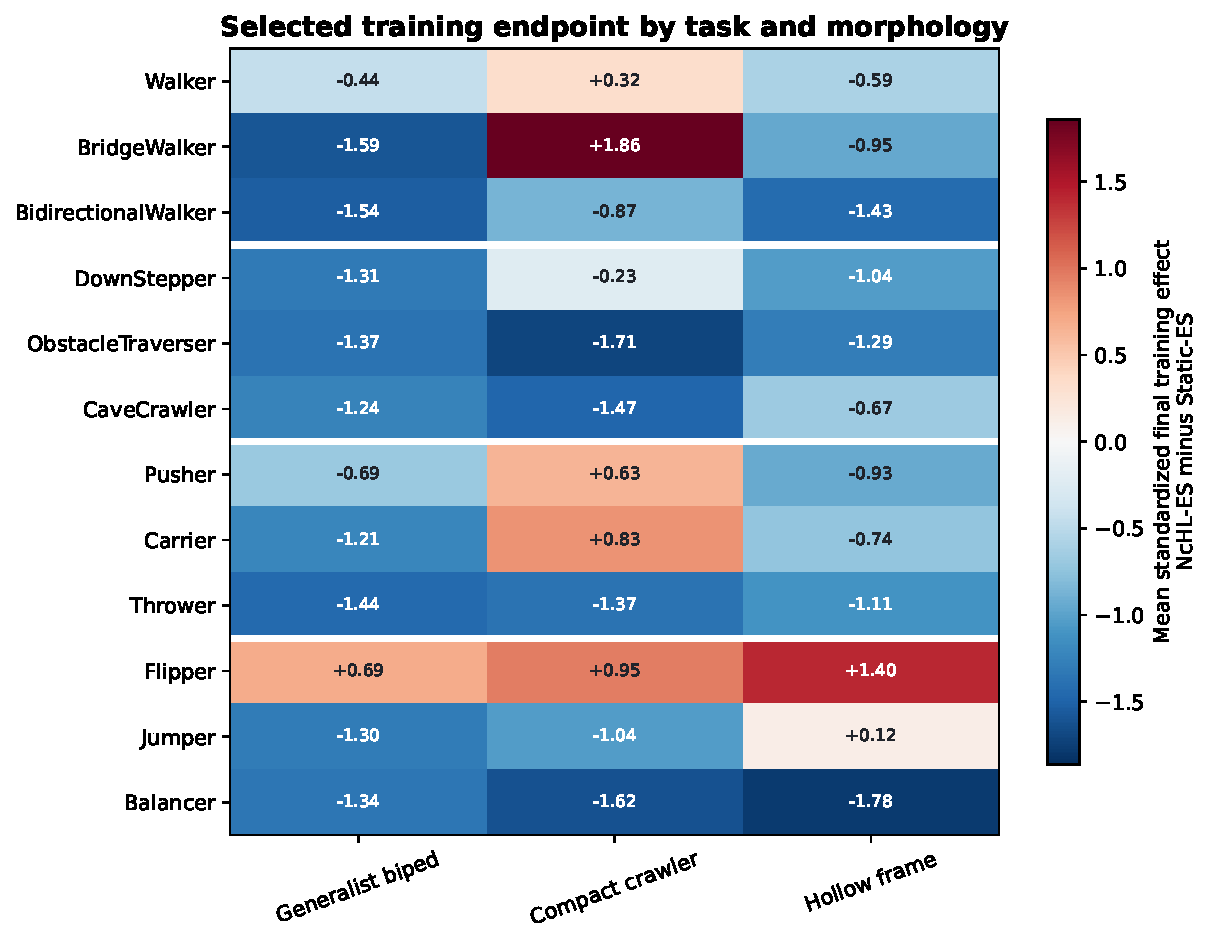
\includegraphics[width=0.86\textwidth]{figures/training_endpoint_heatmap.pdf}
  \caption{Mean standardized final training effect for every task--morphology condition. Positive values favour \nchlcontroller; negative values favour Static-ES. Horizontal separators indicate the four predefined task groups.}
  \label{fig:extended-endpoint-heatmap}
\end{figure}

\Cref{tab:extended-task-effects} summarizes the task averages and the morphology pattern behind them. BridgeWalker illustrates why both levels are required. Its raw task-average score is 6.2\% higher for \nchl{}, but the positive result comes entirely from the compact crawler: its standardized effect is $+1.86$, compared with $-1.59$ for the biped and $-0.95$ for the frame. Seeing as continuous-support locomotion is at least partially learned in the footage, this interaction is behaviourally informative. 

\begin{table}[htbp]
  \centering
  \scriptsize
  \caption{Task-level final training comparison. The raw percentage is meaningful only within its row. The standardized effect averages the three morphology-specific effects.}
  \label{tab:extended-task-effects}
  \begin{tabularx}{\textwidth}{@{}lrr>{\raggedright\arraybackslash}X@{}}
    \toprule
    Task & Raw difference & Mean effect & Morphology pattern \\
    \midrule
    Flipper & $+205.7\%$ & $+1.01$ & Positive for all three bodies \\
    BridgeWalker & $+6.2\%$ & $-0.23$ & Strong crawler advantage; other bodies negative \\
    Walker & $-3.4\%$ & $-0.24$ & Crawler slightly positive; other bodies negative \\
    Pusher & $-5.2\%$ & $-0.33$ & Crawler positive; other bodies negative \\
    Carrier & $-14.4\%$ & $-0.37$ & Crawler positive; other bodies negative \\
    Jumper & $-5.7\%$ & $-0.74$ & Small, inconsistent frame advantage only \\
    DownStepper & $-15.9\%$ & $-0.86$ & Crawler closest to neutral \\
    CaveCrawler & $-1.3\%$ & $-1.13$ & Small but consistent raw disadvantage \\
    BidirectionalWalker & $-47.2\%$ & $-1.28$ & Negative for all three bodies \\
    Thrower & $-19.2\%$ & $-1.31$ & Negative for all three bodies \\
    ObstacleTraverser & $-46.1\%$ & $-1.46$ & Negative for all three bodies \\
    Balancer & $-38.9\%$ & $-1.58$ & Negative for all three bodies \\
    \bottomrule
  \end{tabularx}
\end{table}

\section{Task Characteristics and Answer to RQ4}
\label{sec:extended-interpretation}

\subsection{Favourable and Unfavourable Task Demands}

\paragraph{Continuous-support locomotion.}
This group provides the clearest positive behavioural evidence in the extended suite. The controllers learn the tasks and produce recognizable locomotion. The aggregate group effect still favours Static-ES, so continuous support is not sufficient for an \nchl{} advantage. The more specific pattern is an interaction with body geometry: \nchl{} is positive for the compact crawler on Walker and especially BridgeWalker, but negative for the biped and frame. The evidence therefore supports compatibility between repeated locomotion and a low, stable body rather than a general claim about cyclical movement.

\paragraph{Object interaction.}
The object tasks are also learned recognizably, which makes their score differences relevant. Pusher and Carrier favour \nchl{} with the compact crawler, whereas the other bodies and all Thrower comparisons favour Static-ES. The negative Thrower result may reflect its more specific loading and release demands.

\paragraph{Terrain negotiation.}
The group combines informative and uninformative conditions. DownStepper produces acceptable behaviour and can be interpreted as a genuine controller comparison; its scores favour Static-ES overall, with the crawler closest to neutral. On ObstacleTraverser, Static-ES produces acceptable traversal while \nchl{} fails to perform the task, making this the clearest behavioural disadvantage for \nchl{} in the group. CaveCrawler is learned by neither representation. Its small but consistent numerical difference therefore says little about competent terrain control and should not influence the task-characteristic conclusion strongly.

\paragraph{Whole-body dynamic control.}
None of the Flipper, Jumper, or Balancer controllers learns the intended task recognizably. The apparently strong Flipper score is therefore not evidence that repeated rotation favours \nchl{}. Similarly, the negative Jumper and Balancer effects do not demonstrate that \nchl{} is intrinsically unsuitable for impulse generation or stabilization: the experiment did not first establish successful behaviour with either representation. This group mainly reveals a limitation of the tested morphologies, controller architecture, or training setup.

\subsection{Morphology Dependence}

The compact crawler is the most favourable body numerically, with a mean effect of $-0.31$ across tasks, compared with $-0.75$ for the hollow frame and $-1.07$ for the biped. More importantly, its positive results on Walker, BridgeWalker, Pusher, and Carrier occur in the two groups where the footage shows recognizable task learning. For continuous-support locomotion, the crawler effect is $+0.44$ with a 95\% interval of $[+0.27,+0.62]$, and every seed-level group average is positive. Its low rectangular geometry and broad contact area may permit useful repeated deformation without the same balance and foot-placement demands as the biped or frame.

The positive Flipper cell is excluded from this behavioural argument because the task is not learned. Even after that exclusion, the remaining informative positive cells are concentrated in the crawler. The evidence therefore indicates a task--body interaction rather than a task characteristic that operates independently of morphology. The three selected bodies cannot identify whether contact area, height, mass distribution, or another geometric property is responsible.

\subsection{RQ4 Summary}

The experiment does not identify a broad task characteristic that makes \nchl{} consistently successful. The most credible positive evidence occurs in partially learned continuous-support and object-interaction tasks when they are paired with the compact crawler. 

The observed pattern is therefore strong morphology-dependency. NcHL may be compatible with repeated locomotion or sustained contact when the body supplies a stable mechanical foundation, but the current evidence does not establish an advantage for cyclicality, rotation, impulse generation, or stabilization as general task properties. 
